% Section 5: Chapter 3 - Real-World Applications
% Division: 5.1 (Member B - Nguyen Tien Cuong); 5.2 (Member A - Pham Tran Anh Quan).
\section{Chapter 3: Real-World Applications}
\label{sec:05_chapter3_applications}

All frequent itemsets and association rules analyzed in this chapter are mined exclusively using our \texttt{EclatFIM} implementation, without invoking any external frequent itemset mining library.

% ---------------------------------------------------------------------------
\subsection{Application 1: Market Basket Analysis on the Groceries Dataset}
\label{subsec:app1_groceries}

\subsubsection{Problem Formulation and Data Transformation Analysis}
Market basket analysis is conducted on the \texttt{Groceries} retail dataset from the \texttt{arules} package~\cite{hahsler2005arules}, comprising $N = 9{,}835$ point-of-sale transactions across $m = 169$ named product items. Unlike anonymized datasets such as \texttt{Retail}, explicit product names in \texttt{Groceries} allow direct domain interpretation. Each receipt is converted into an SPMF-formatted transaction accompanied by \texttt{@ITEM=id=name} metadata lines; \texttt{read\_spmf} ignores metadata directives during mining and maps item codes back to product names for rule interpretation.

To evaluate how transaction granularity affects Eclat's behavior, two transformation schemes are compared at $\texttt{minsup} = 1\%$ ($\sigma_{\min} = 99$) and $\texttt{minconf} = 0.3$: (i) retaining all $169$ fine-grained product items, and (ii) aggregating items into $12$ coarse supermarket categories (such as \texttt{dairy\_eggs}, \texttt{produce}, \texttt{bakery}, and \texttt{meat\_seafood}). Table~\ref{tab:b08_groceries_transform} highlights two key findings:
\begin{itemize}
    \item Under the fine-grained $169$-item representation, the average density is $\rho = \bar{L}/m = 2.61\%$, closely approaching the theoretical $1/32 \approx 3.125\%$ crossover threshold between \texttt{Vector\{Int32\}} and \texttt{BitVector} tidset representations in Eclat. With short transactions ($\bar{L} = 4.41$), mining completes in $0.0256$~s and yields $125$ actionable rules.
    \item Aggregating into $12$ coarse categories increases density nearly tenfold to $25.98\%$, expanding the pattern space from $333$ to $477$ frequent itemsets and causing rule volume to surge to $2{,}232$ overly generic rules (e.g., \emph{dairy $\Rightarrow$ produce}) that offer limited merchandising utility. Consequently, the $169$-item representation is selected.
\end{itemize}

% Data source: results/groceries_b08_transforms.csv
\begin{table}[H]
\centering
\caption{Quantitative comparison of two Groceries transformation schemes at $\texttt{minsup} = 1\%$, $\texttt{minconf} = 0.3$ (variant \texttt{v1}).}
\label{tab:b08_groceries_transform}
\begin{tabular}{lrrrrrr}
\toprule
Representation Scheme & $m$ & $\bar{L}$ & $\rho$ & $|\mathcal{F}|$ & Rules & Runtime \\
\midrule
169 original items (selected) & 169 & 4.41 & 2.61\% & 333 & 125 & 0.0256 s \\
12 coarse product categories & 12 & 3.12 & 25.98\% & 477 & 2,232 & 0.0024 s \\
\bottomrule
\end{tabular}
\end{table}

\subsubsection{Threshold Sensitivity Analysis}
Rule sensitivity is evaluated over the parameter grid $\texttt{minsup} \in \{0.5\%, 1\%, 2\%\} \times \texttt{minconf} \in \{0.2, 0.3, 0.5\}$ (\texttt{results/groceries\_grid.csv}). At $\texttt{minsup} = 0.5\%$ ($\sigma_{\min} = 50$), the algorithm produces $1{,}001$ frequent itemsets and up to $893$ rules (at $\texttt{minconf} = 0.2$), introducing numerous low-evidence associations. Conversely, at $\texttt{minsup} = 2\%$ ($\sigma_{\min} = 197$), only $37$ rules remain at $\texttt{minconf} = 0.3$ (and a single rule at $0.5$), pruning specialized purchasing patterns. Selecting $\texttt{minsup} = 1\%$ ($\sigma_{\min} = 99$) and $\texttt{minconf} = 0.3$ yields $125$ rules, striking a balanced trade-off between coverage and interpretability.

\subsubsection{Primary Results and Business Interpretation}
Figure~\ref{fig:f11_groceries} maps all $125$ rules across support and confidence, color-coded by lift. Ranking by confidence alone exhibits strong popularity bias: \texttt{whole milk} appears in $2{,}513/9{,}835$ baskets ($25.55\%$), causing top-confidence rules to predominantly feature \texttt{whole milk} as the consequent despite modest lift (e.g., \texttt{curd + yogurt} $\Rightarrow$ \texttt{whole milk} achieves $\text{conf} = 0.582$ with $\text{lift} = 2.279$). Ranking by lift~\cite{brin1997dynamic} adjusts for baseline prevalence and surfaces genuine co-purchasing affinities (Table~\ref{tab:b09_groceries_top10}).

\begin{figure}[H]
\centering
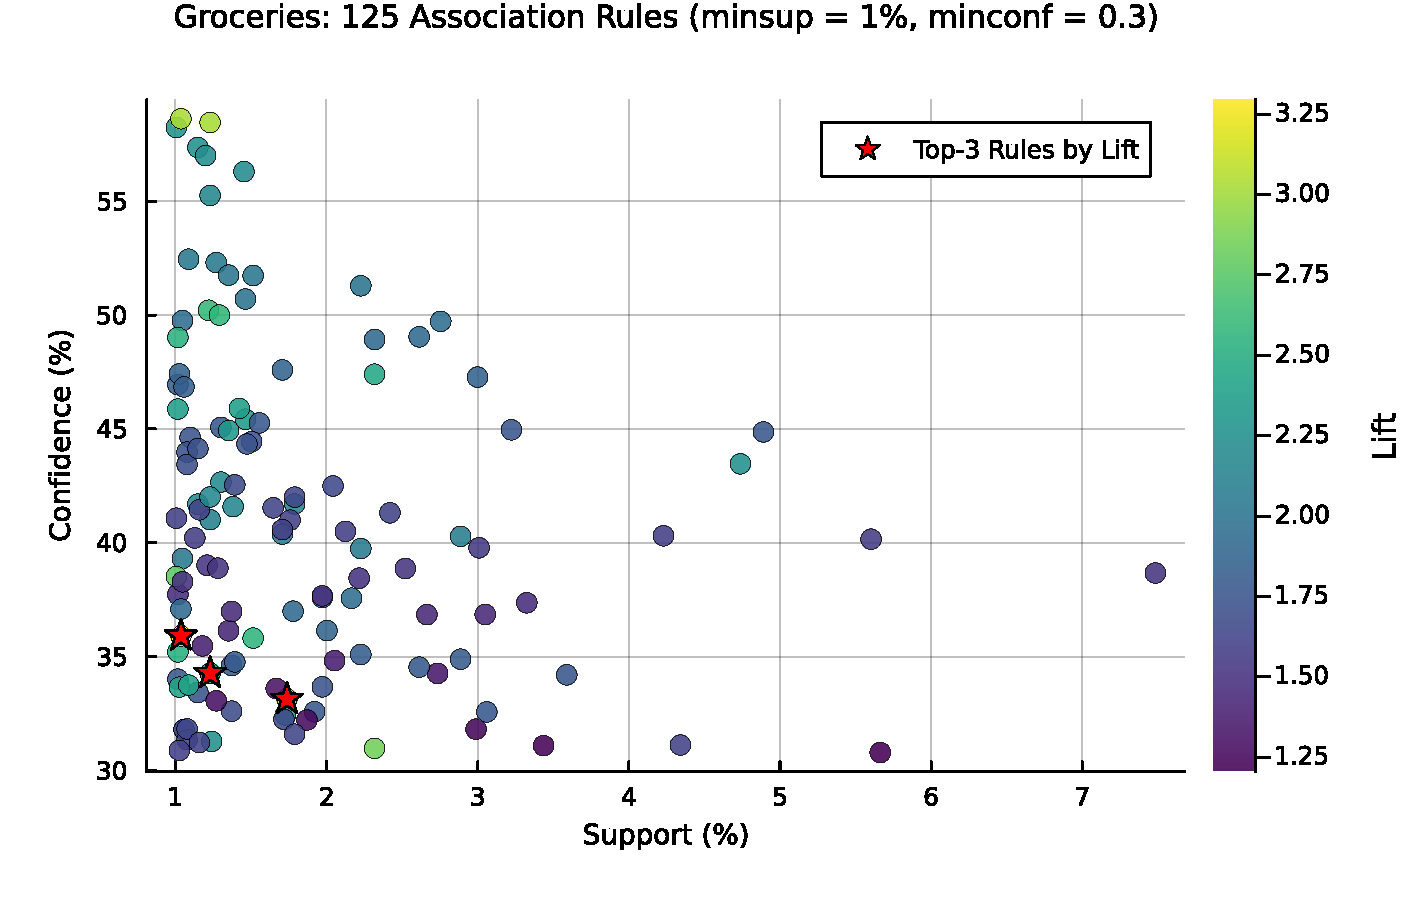
\includegraphics[width=0.88\textwidth]{F11_groceries_rules.pdf}
\caption{Distribution of $125$ association rules on the Groceries dataset ($\texttt{minsup} = 1\%$, $\texttt{minconf} = 0.3$) across support and confidence, colored by lift; red stars denote the top-3 rules by lift.}
\label{fig:f11_groceries}
\end{figure}

% Data source: results/groceries_top10.csv
\begin{table}[H]
\centering
\caption{Top-10 association rules ranked by lift on the Groceries dataset ($\texttt{minsup} = 1\%$, $\texttt{minconf} = 0.3$).}
\label{tab:b09_groceries_top10}
\begin{tabular}{rllrrrr}
\toprule
Rank & Antecedent ($X$) & Consequent ($Y$) & $\sigma$ & Support & Confidence & Lift \\
\midrule
1 & citrus fruit + other vegetables & root vegetables & 102 & 0.0104 & 0.3592 & 3.295 \\
2 & other vegetables + tropical fruit & root vegetables & 121 & 0.0123 & 0.3428 & 3.145 \\
3 & beef & root vegetables & 171 & 0.0174 & 0.3314 & 3.040 \\
4 & citrus fruit + root vegetables & other vegetables & 102 & 0.0104 & 0.5862 & 3.030 \\
5 & root vegetables + tropical fruit & other vegetables & 121 & 0.0123 & 0.5845 & 3.021 \\
6 & other vegetables + whole milk & root vegetables & 228 & 0.0232 & 0.3098 & 2.842 \\
7 & curd + whole milk & yogurt & 99 & 0.0101 & 0.3852 & 2.761 \\
8 & rolls/buns + root vegetables & other vegetables & 120 & 0.0122 & 0.5021 & 2.595 \\
9 & root vegetables + yogurt & other vegetables & 127 & 0.0129 & 0.5000 & 2.584 \\
10 & tropical fruit + whole milk & yogurt & 149 & 0.0151 & 0.3582 & 2.568 \\
\bottomrule
\end{tabular}
\end{table}

The top rules in Table~\ref{tab:b09_groceries_top10} reveal three actionable consumer clusters:
\begin{itemize}
    \item \textbf{Home-Cooking Ingredients (Rank~3):} Customers purchasing \texttt{beef} buy \texttt{root vegetables} at $3.04\times$ the baseline rate ($\sigma = 171$), reflecting meal-preparation habits (e.g., stews and soups). Placing fresh root vegetables adjacent to the meat counter or offering bundled meal kits directly leverages this affinity.
    \item \textbf{Fresh Produce Cluster (Ranks~1, 2, 4, 5):} \texttt{citrus fruit}, \texttt{tropical fruit}, \texttt{other vegetables}, and \texttt{root vegetables} exhibit strong mutual reinforcement ($\text{lift} > 3.0$), supporting contiguous produce layouts and multi-item produce promotions.
    \item \textbf{Dairy Cluster (Ranks~7, 10):} \texttt{curd + whole milk} $\Rightarrow$ \texttt{yogurt} ($\text{lift} = 2.761$) supports cross-promotional placement within refrigerated dairy aisles.
\end{itemize}

\subsubsection{Out-of-Sample Stability Evaluation (80/20 Split)}
Rule generalizability is assessed via a reproducible $80\%/20\%$ random split (\texttt{seed} $= 42$), yielding $N_{\text{train}} = 7{,}868$ training baskets and $N_{\text{test}} = 1{,}967$ test baskets. The top-10 rules by lift mined on the training split are re-evaluated on the held-out test split (Table~\ref{tab:b10_groceries_stability}). All $10/10$ rules preserve $\text{test\_lift} > 1.5$. Core associations such as Rank~1 ($-4.5\%$ shift), Rank~5 ($-3.4\%$), and Rank~4 (\texttt{beef} $\Rightarrow$ \texttt{root vegetables}, $-8.5\%$) demonstrate high stability, whereas Rank~6 (\texttt{whipped/sour cream + whole milk} $\Rightarrow$ \texttt{root vegetables}) experiences a $-38.3\%$ drop due to higher sampling variance near the $1\%$ support boundary.

% Data source: results/groceries_stability.csv
\begin{table}[H]
\centering
\caption{Stability evaluation of top-10 training rules by lift on an $80/20$ split (\texttt{seed} $= 42$, $N_{\text{train}} = 7{,}868$, $N_{\text{test}} = 1{,}967$).}
\label{tab:b10_groceries_stability}
\begin{tabular}{rlrrr}
\toprule
Rank & Rule ($X \Rightarrow Y$) & Train Lift & Test Lift & Shift \\
\midrule
1 & citrus fruit + other vegetables $\Rightarrow$ root vegetables & 3.325 & 3.175 & $-4.5\%$ \\
2 & other vegetables + tropical fruit $\Rightarrow$ root vegetables & 3.242 & 2.734 & $-15.7\%$ \\
3 & citrus fruit + root vegetables $\Rightarrow$ other vegetables & 3.159 & 2.568 & $-18.7\%$ \\
4 & beef $\Rightarrow$ root vegetables & 3.093 & 2.831 & $-8.5\%$ \\
5 & root vegetables + tropical fruit $\Rightarrow$ other vegetables & 3.040 & 2.935 & $-3.4\%$ \\
6 & whipped/sour cream + whole milk $\Rightarrow$ root vegetables & 2.925 & 1.805 & $-38.3\%$ \\
7 & other vegetables + yogurt $\Rightarrow$ root vegetables & 2.864 & 2.203 & $-23.1\%$ \\
8 & other vegetables + whole milk $\Rightarrow$ root vegetables & 2.787 & 3.072 & $+10.2\%$ \\
9 & other vegetables + whipped/sour cream $\Rightarrow$ yogurt & 2.612 & 2.214 & $-15.3\%$ \\
10 & rolls/buns + root vegetables $\Rightarrow$ other vegetables & 2.588 & 2.628 & $+1.5\%$ \\
\bottomrule
\end{tabular}
\end{table}

\subsubsection{Limitations and Practical Extensions}
Three methodological limitations warrant caution when operationalizing association rules: (i) high-lift rules with support near the minimum threshold rest on limited sample evidence and exhibit higher out-of-sample variance; (ii) lift is symmetric ($\text{lift}(X \Rightarrow Y) = \text{lift}(Y \Rightarrow X)$) and therefore does not identify purchase directionality; and (iii) co-occurrence does not imply causality, as unobserved confounders such as weekend shopping cycles or seasonality may drive joint demand. In practice, stable rules can feed real-time e-commerce basket recommenders or generate hypotheses for controlled A/B shelf-placement experiments.

% ---------------------------------------------------------------------------
\subsection{Application 2: Visual Pattern Discovery via Bag of Visual Words}
\label{subsec:app2_bovw}
% To be completed by Member A (Caltech-101, Tables B11-B13, Figures F12-F13).
